\pdfoutput=1

\documentclass{l4proj}
\usepackage{url}
\usepackage{subcaption}
\usepackage{float}
% compacting the list items
\usepackage{enumitem}

%
% put any packages here
%

\begin{document}
\title{Urban Data Timeline}
\author{Yordan Yordanov}
\date{March 28, 2016}
\maketitle

\begin{abstract}
We show how to produce a level 4 project report using latex and pdflatex using the 
style file l4proj.cls
\end{abstract}

\educationalconsent
%
%NOTE: if you include the educationalconsent (above) and your project is graded an A then
%      it may be entered in the CS Hall of Fame
%
\tableofcontents
%==============================================================================

\chapter{Introduction}
\pagenumbering{arabic}

\section{Background}

Smart cities today represent a perception to integrate both information and communication technologies in an acceptable and maintainable fashion to manage their infrastructure and facilities. The optimal goal is to enhance the quality of life and satisfy the residents’ needs. ICT gives to the people, who maintain these cities, the great opportunity to directly follow what is happening and take actions accordingly. This can be done only by processing the huge amounts of information, collected from sensors, in real time and providing knowledge and information – the keys for discovering inefficiencies. 

However, the biggest asset of a smart city is not the number of cameras or sensors but the people that occupy it. A third of the internet users (Ofcom’s 2015 communications marker report, published on 6 August) represent their smartphone as the most important device for going online. A third of the population owns a smart device and use it every day to bank, shop and access social media. Social media streams, such as Twitter, have a reputation to be extremely useful source of information. Anybody can understand what is happening all around the world in real time. With that comes various opportunities for developers to implement systems that automatically detect and track events as they happen. Smart cities can benefit from that as what better way to improve efficiency than for example identifying and reporting road accidents to the emergency services.

Aiming to help with analyzing these massive amounts of data, the Urban Big Data Centre was established by the UK Economic and Social Research Council to address social, economic and environmental challenges facing cities. Their researchers are undertaking innovative projects, covering topics from big data management to linking and analysing the multi-structural urban data.  Such project is the Integrated Multimedia City Data. 



\subsection{Integrated Multimedia City Data\cite{imcd}}


Integrated Multimedia City Data (iMCD) is one of the Urban Big Data Centre’s inaugural projects, funded by the Economic and Social Research Council. It is designed to provide the UBDC with innovative primary data sources. The project consists of four strands: representative household survey, tracking of real-time urban sensors, internet based visual media collection and internet based textual media collection.  

The core research strand is the representative household survey that aims to gather data about people’s attitude and behaviour when it comes to information and communication technologies, traveling and learning. Part of the participants are given GPS and life logging sensors that will record their activities and travel. Meanwhile the visual and textual data, referring to Glasgow and surrounding areas, is to be collected from the internet. All of it together is able to show how Glasgow performs as a smart city.  The Terrier IR team provides various data web services so that all these sources can be browsed and queried.


\subsection{Web Services}

Describe what a web service is

\subsection{Web Application}

Describe what a web application is

\section{Aims}

This project aims to build a tool for the fusion and visualisation of timely data collected from the UBDC for their project, described earlier (iMCD). Past data from various urban data streams, such as social media posts, news, blogs, traffic information, environmental sensors and many more has been provided. The tool should be able to query all this data and come up with a timeline representation of observations that might be of interest to the user. This application is initially build to be used by the \textbf{general public} but may as all be valuable to local researchers who follow or compare people’s opinions, businessmen who want to know how their business is developing, media that want to report what are the public impressions about an important event and even politicians while running their campaigns.   

\section{Motivations}

Smart cities bring a lot of advantages. They can opt for better urban planning and development by making more efficient use of the infrastructure to improve productivity and services but also to reduce the waste of fuel and energy. Furthermore their intelligence can change and enhance the way authorities respond to changing circumstances. On the other hand, achieving all these goals is a challenging process. Huge amounts of information, created by social feeds, environmental sensors, traffic, news and many more, have to be gathered, stored and analysed. This project aims to combine and visualise all these data strands so that some can look at the cities from a different angle and possibly extract new tendencies and patterns, not possible to discover by following only a single resource. This will help us identify problems or challenges that we had not been aware of and provide effective solutions that we all as citizens can only benefit from. (maybe add something for releasing this tool to the general public)

\chapter{Related Work}
There are applications that have been developed to accomplish similar if not the same goals, but most of them are concentrating on a single data stream. This chapter is presenting a short description of related products, along with key differences and correlations in comparison with the goals of this project.   

\textbf{Google Maps Timeline \cite{GoogleMapsTimeline}}

Google stores a history of where anybody that uses its location services goes. All this data is collected by your device sensors and the navigation you use and then visualized with the Google Maps Timeline feature. It is advertised to be an easy way to view and remember places somebody has been on a given day at a given time. Without any input, the timeline shows predictions of when you have arrived or left a place. One of the key features is highlighting when you have visited the most places and how you had travelled. The application does not offer sharing as Google wants your information to remain private. As far as human interaction goes, you are allowed to correct, confirm or delete a place where Google thinks you had been but even after deleting,  it can still be seen that you had passed by that area. In 2009, the company released a similar feature called Google Latitude that offered sharing of location history but the project was closed down \cite{GMTimeFeature}.


This product has the same initial goal to visualize timely data originating from different streams like navigation history, pictures, travel and walking routes. However what it has in common is it uses a vertical timeline to display the events, it allows searching based on a specific day, month, year and has a way to show (via bar chart) how active you have been every day in the past few weeks. 

\textbf{Social Media Timeline}

All social media websites in the likes of Twitter and Facebook use some sort of a timeline to visualize their user's personal information. However they differ on the way they organize their posts. Facebook describes a timeline to be a place on your profile where you can see your own posts, your friends' activities and stories you're tagged in, sorted by the date and time they were posted. On the other hand, Twitter displays a stream of tweets from accounts that you have chosen to follow. Making use of machine learning algorithms, posts that you are likely to care about more are displayed first.


Despite of the fact that social media applications has as a main goal the delivery of a secure and reliable tool for communication, they also provide their users with the ability to visualize their personal data streams like photos, events, group activities and accomplishments. Both Facebook and Twitter use a vertical timeline and allow for searching based on keywords. One of the key features is infinite scrolling that make the illusion of one endless stream of events by making use of the million users, posting every day. 

\chapter{Project Planning}

\section{Project Management}

When a new product is developed, it is not clear how it will end up and if it will fulfil the user's requirements. The developers can see the first steps but there are plenty of problems or challenges that can not be predicted from the beginning (Figure \ref{projectInitial}). That is true for any project, no matter how much planning is put in. However there is a possibility that everything is done the right way but there is a high probability to drift away from the initial target (Figure \ref{projectStart}). There are several methodologies that can be followed when developing a software but the two most common are Waterfall and Agile. 

The Waterfall model is an example of a plan-driven process - in principle you must plan and schedule all of the process activities before starting work on them \cite{sene}. Here iterations can be costly and involve significant rework. Therefore, after a small number of iterations, it is normal to freeze parts of the development, such as the specification, and continue with the later development stages. Problems are left for later resolution, programmed around or completely ignored. This implementation tricks may also lead to design problems and badly structured systems.

This project, on the other hand, follows the Agile methodology (Figure \ref{projectAgile}) for software development. It is an interactive
approach that splits the work into a number of iterations (sprints). This allow the project supervisors to inspect the work of the developer and monitor how well the software development is progressing \cite{sene}. Each of these sprints last one
week. It starts with a meeting and demonstration of the work done in the previous sprint. As an
outcome of these meetings feedback from the supervisors is received, based on the
extent to which their requirements are met. Moreover, these meetings allow discussions of the issues
that are experienced and compare the available workarounds. At the end of a meeting, it is agreed
upon exactly what work will be done during the next sprint. Following this scenario, at least one new
feature is introduced after each sprint and changes to previous features are performed as early as possible. By the end of this project, 23 iterations are to be performed.

\begin{figure}[H]
\begin{subfigure}{.3\textwidth}
	\centering
	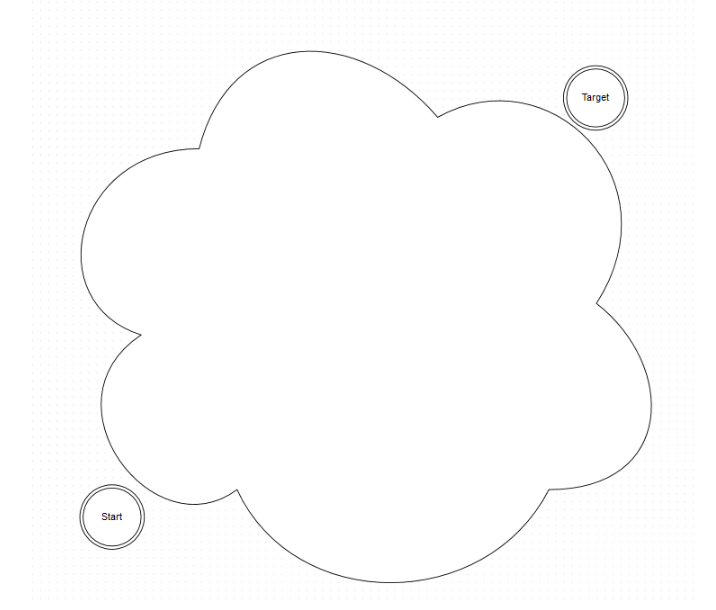
\includegraphics[height=4cm,width=4cm]{images/projectInitial}
	\caption{Start of a project.}
	\label{projectInitial}
\end{subfigure}
\begin{subfigure}{.3\textwidth}
	\centering
	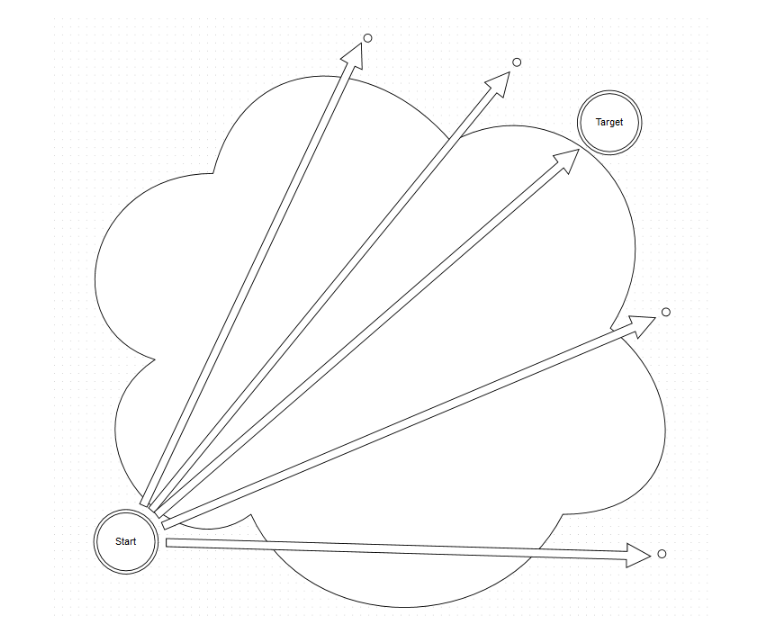
\includegraphics[height=4cm,width=4cm]{images/projectStart}
	\caption{Waterfall methodology.}
	\label{projectStart}
\end{subfigure}
\begin{subfigure}{.3\textwidth}
	\centering
	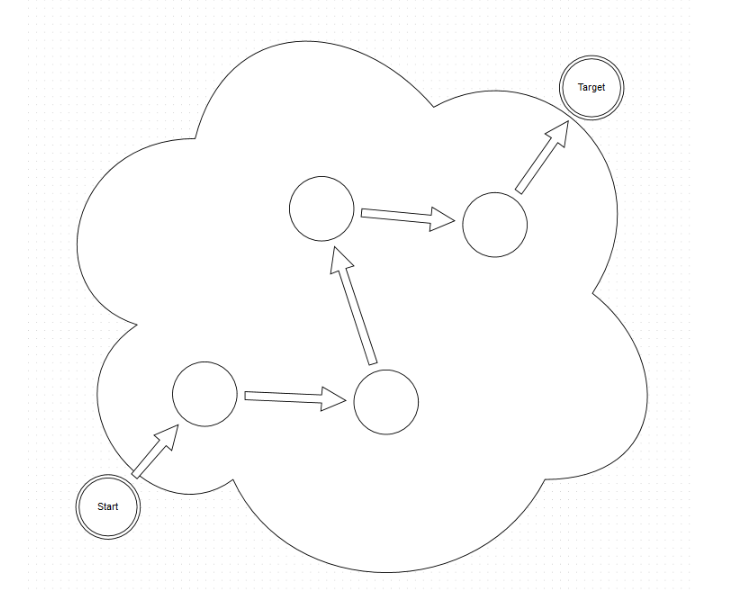
\includegraphics[height=4cm,width=4cm]{images/projectAgile}
	\caption{Agile methodology.}
	\label{projectAgile}
\end{subfigure}
\end{figure}



\section{Requirements Engineering}

The requirements for a system describes the functionality of the services it provides and the constraints of its operation. The process of gathering, analysing and documenting these services and constraints is called requirements engineering.

At the beginning of the project, a few weeks were taken to envision the high-level requirements and to understand the scope of the required system. For the initial requirements use cases and user stories to help with exploring how users will work with the system. 

\subsection{Use cases} 

Use case is a way to describe how a real user interacts with the system. They should not be perfect and can only show the action and not go into much detail, in order to stay close to the agile methodology. The developer will implement the system but will have to work close with the supervisors so that the end product will meet their needs. 

The following use cases were identified in the beginning of this project: 


\begin{itemize}%[noitemsep]
	\item see how tweets about a specific hashtag are distributed over a period of time
	\item see popular hashtags that are twitted together with a specific hashtag
	\item get information about a certain area of the city and find out if the venues(restaurants, train stations, cinemas) there get high attendance
	\item browse tweets based on time and hashtag
	\item use the system on a mobile device
	\item check out what the clients post about a venue, they had visited
	\item check how many people attend specific venues in a given area
	\item compare people's opinions about an event
	\item see if a political party is likely to win the elections
\end{itemize}


\subsection{User Stories}

User stories are one of the primary development artefacts for Agile project teams. A user story is a high-level definition of a requirement, containing just enough information so that the developers can get a feel of what the user wants to achieve when using the system by performing a task. It represents a functionality that will be of a value to the user. A suggested template for a user story is: 

	\begin{center}
		As a \textbf{\textit{ROLE}}, I want to \textbf{\textit{ACTION}}, so that \textbf{\textit{GOAL}}. \cite{sets}
	\end{center}

The role represents the user that interacts with the system. The action shows how the user wants to use the system and the goal- what the user is trying to accomplish. All user stories are written in a way that they are understandable by both developer and customer. Ideally the customer should write the user stories while discussing them with the developer \cite{sets}. The following list represents the user stories, captured for this project based on the identified target users(TODO: should I talk about target users):    

\begin{itemize}%[noitemsep]
	\item \textbf{\textit{Researcher}}.
	\begin{itemize}
		\item As a Researcher, I would like to see how the tweets for certain query are distributed though out a period of time, so that I can see the pick of the number of tweets.
		\item As a Researcher, I would like to know other popular twitter hashtags for a certain day, so that I can see what was interesting for the Twitter users for that day.
		\item As a Researcher, I would like to know if specific area of the city was busy on a specific date, so that I can see if specific event or weather conditions had affected that area.
		\item As a Researcher, I would like to see a timeline representation of the tweets for a specific query, so that I can follow and see if the user’s opinions change.
		\item As a Researcher, I would like to use the app on a mobile device, so that when I travel, I can continue working on my research.
		\item As a Researcher, I would like to know what were the weather conditions on a specific date and see traffic information, so that I can use the data as an experiment and measure the likelihood of using the public transport when the weather conditions are bad. 
	\end{itemize}
	
	\item \textbf{\textit{Business owner}}.
	\begin{itemize}
		\item As a Restaurant owner, I would like to see if posting a tweet on my timeline affects the number of people that attend my restaurant.
		\item As a Restaurant owner, I would like to see other venues in my area, so that I can check their attendance and try to improve mine.
		\item As a TV channel owner, I would like to compare how many people are talking about my channel at specific time, compared to other channels so that I can change my TV guide and increase my audience.
	\end{itemize}
	
	\item \textbf{\textit{Politician}}.
	\begin{itemize}
		\item As a politician, I would like to compare how popular is my party in the social media in comparison to other parties, so that I can change my campaign and increase my chances of winning.
	\end{itemize}
	
	\item \textbf{\textit{Citizen}}.
	\begin{itemize}
		\item As a citizen, I would like to compare two different public opinions about a specific event, so that I can make a decision of my own. 
	\end{itemize}
\end{itemize}

\subsection{Functional requirements} 

Functional requirements represent services the system should provide, how it should react to particular inputs and how the system should behave in some situations. More specific requirements can describe the system functions, its inputs and output or exceptions in detail \cite{sene}. 

Adding new requirements may change the project direction. Projects usually have fixed duration so sometimes it may not be possible to include all the features. Therefore all use cases that are identified in this chapter must be prioritised. 

Figure \ref{MoSCoW} shows the MoSCoW rules that are typically used as a guideline for prioritising requirements. All the use cases should be sorted, using these rules. The ones that are "Must Have" and "Should Have" should be feasible in the duration of the project. The following list represents the extracted requirements after their prioritisation.

\begin{figure}[H]
	\centering
	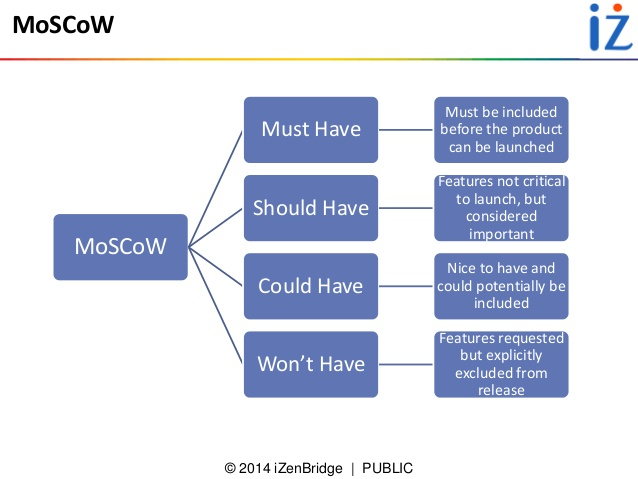
\includegraphics[height=6cm,width=8cm]{images/MoSCoW}
	\caption{MoSCoW rules prioritisation scheme for requirements}
	\label{MoSCoW}
\end{figure} 

\textbf{\textit{Functional Requirements}}.
\begin{itemize}
	\item \textit{User Interface}
	\begin{itemize}
		\item Must be able to display a fusion of different kinds of timely data (tweets, weather, traffic, train delays etc.).
		\item Must be able to show specific as well as general information based on the request.
		\item Must display events in a timeline.
		\item Must display the time of events.
		\item Must be able to take date input.
		\item Must be able to receive hashtag input.
		\item Must be able to take location based input.
		\item Must be able to show venues in specific area. (using a Map)
		\item Should dynamically add data to the layout. (using AJAX)
		\item Should be able to visualise statistic data on a graph.
		\item Could show a summary of the made request.
		\item Could show the link of an event with other events.
	\end{itemize}
	
	\item \textit{Server}
	\begin{itemize}
		\item Must be able to fetch data from provided services.
		\item Must be able to fetch data from external sources. (Twitter)
		\item Should provide additional RESTful APIs. (TODO: explain what is REST)
		\item Should support caching.
		\item Could store pre-render events. 
		
	\end{itemize}
\end{itemize}   


\subsection{Non-Functional requirements}

Non-functional requirements represent constraints on the services or functions offered by the system. They often apply to the application as a whole, rather than individual components \cite{sene}.

	\textbf{\textit{Non-Functional Requirements}}.
	\begin{itemize}
		\item Must be universal to support all kinds of users(citizen, scientist, researchers, local authorities)
		\item Must be extensible so that different things can be rendered on the views.
		\item Must be able to quickly process the data from the services.
		\item Should be accessible from and compatible with desktops, laptops, tablets and smartphone devices.
		\item Should be testable.
		\item Should be scalable so that new services can be added.
		\item Could be compatible with code quality tools. (Sonar)
	\end{itemize}


\chapter{Design}

\chapter{Solution}

\section{Choice of technology}

\section{Components communication}

\chapter{Components}

\section{Model}

\section{View}

\section{Controller}

\section{Challenges}

\chapter{Evaluation}

\section{Product evaluation}

\subsection{Initial phase}

\subsection{Final phase}

\section{Testing}

\chapter{Future work}

%%%%%%%%%%%%%%%%
%              %
%  APPENDICES  %
%              %
%%%%%%%%%%%%%%%%
\begin{appendices}

\chapter{Running the Programs}
An example of running from the command line is as follows:
\begin{verbatim}
      > java MaxClique BBMC1 brock200_1.clq 14400
\end{verbatim}
This will apply $BBMC$ with $style = 1$ to the first brock200 DIMACS instance allowing 14400 seconds of cpu time.

\chapter{Generating Random Graphs}
\label{sec:randomGraph}
We generate Erd\'{o}s-R\"{e}nyi random graphs $G(n,p)$ where $n$ is the number of vertices and
each edge is included in the graph with probability $p$ independent from every other edge. It produces
a random graph in DIMACS format with vertices numbered 1 to $n$ inclusive. It can be run from the command line as follows to produce 
a clq file
\begin{verbatim}
      > java RandomGraph 100 0.9 > 100-90-00.clq
\end{verbatim}
\end{appendices}

%%%%%%%%%%%%%%%%%%%%
%   BIBLIOGRAPHY   %
%%%%%%%%%%%%%%%%%%%%

\bibliographystyle{plain}
\bibliography{bib}

\end{document}
